\documentclass[a4paper, 12pt]{article}
\usepackage[utf8]{inputenc}
\DeclareUnicodeCharacter{2074}{\ensuremath{{}^4}}
\usepackage{listings}
\usepackage{graphicx}
\title{Obligatorisk innlevering 2}
\author{Sivert M. Skarning}
\date{Mai 2019}
\begin{document}
\maketitle

\section{Oppgave 2}
\subsection{Oppgavebeskrivelse}
I denne oppgaven skal dere sammenligne ulike kantdeteksjonsalgoritmer. Det er her lov å ta i bruk innebygde implementasjoner. Dere må teste minst tre ulike algoritmer og dere skal teste med ulike verdier for konstanter slik som sigma og threshold. Resultatet skal vises frem og diskuteres.

\subsection{Dokumentasjon}
I denne oppgaven valgte jeg tre kantdeteksjons algoritmer.
\begin{itemize}
\item Sobel operator
\item Prewitt operator
\item Canny kantdetektor
\end{itemize}

For canny algoritem prøvde jeg med tre verdier for standardavvik på det Gaussiske filteret, 1, 5 og 20. Selvom jeg implementerte canny algoritmen i forrige oppgave valgte jeg å bruke en innebygd versjon fordi jeg ikke var helt fornøyd med resultatet. Den innebygde algoritmen fungerer bra å her enkel å bruke. Det er derimot ikke mulig å endre tresholdene på hysteresis tresholding.

\subsection{Resultat}
\paragraph{Canny kantdetektor}I figur \ref{fig:canny} ser dere tre bilder. Disse bildene er resultatet av en Canny kantdetektor. Forskjellen på bildne er standardavvik brukt på den Gaussiske utjevningen. Fra venstre ser dere resultatet med standardavvik på 1, 5 og 20. Med 20 som standardavvik blir bildet såpass utjevnet at Canny algoritmen ikke finner noen kanter i bilde. Følgelig blir hele blidet svart. På bildet med 1 i standardavvik ser man at alle kanter i bildet fremkommer. Med 5 i standardavvik er det kun de klareste kantene som kommer med. Dette resultatet er ønskelig da det er lett å velge filtrere ut de kantene som man annser som støy. Ved hjelp av å variere utjevningen kan man få fram ulike karakteristikker i bilde etter behov.

\paragraph{Sobel og Prewitt kantdetektor}
I figur \ref{fig:sobprew} ser man resultatet av sobel operatorene i midten og prewitt operatoren til høyre. I figur \ref{fig:mat} ser man at man trenger to sett med operatorer. En som går i x-retning og en som går i y-retning. Hvis man konvolverer et bilde med disse filterene får man kantene i x-retning og kantene i y-retning. Hvis man legger dette sammen får man kantene alle kantene i bilde.
Som man ser i figur \ref{fig:sobprew} er det ingen forskjell mellom Sobel og Prewitt operatorene for dette bilde. Det som er hovedforskjellen er at sobel koeffisientene kan endres etter behov, det kan man ikke med prewitt operatorene \footnote{https://www.quora.com/What-is-the-basic-difference-between-Sobel-Operator-and-Prewitt-operator}

\paragraph{Canny vs Sobel/Prewitt}
Forskjellen mellom canny kantdetektoren og Sobel/Prwitt kantdetekteringen er stor. Det første man legger merke til er hvor tynne og hvor tydlig kantene er på figur \ref{fig:canny} i forhold til på figur \ref{fig:sobprew}. De tynne kantene kommer fra non-max supression delen i Canny algoritmen. Her går man gjennom alle kantene å sjekker etter lokale maxima. Kantene blir tydligere på grunn av Hysteresis Tresholding. Her går man gjennom kantene og gjør de monokrome, man eliminerer også de pixelene som ikke er en del av en større kant for ikke å få med støy. Alt dett gjør at Canny kantdetektoren generelt er et bedre valg en Sobel/Prewitt avhengig av hvilke karakteristikker man er ute etter.


\begin{figure}[h]
  \centering
  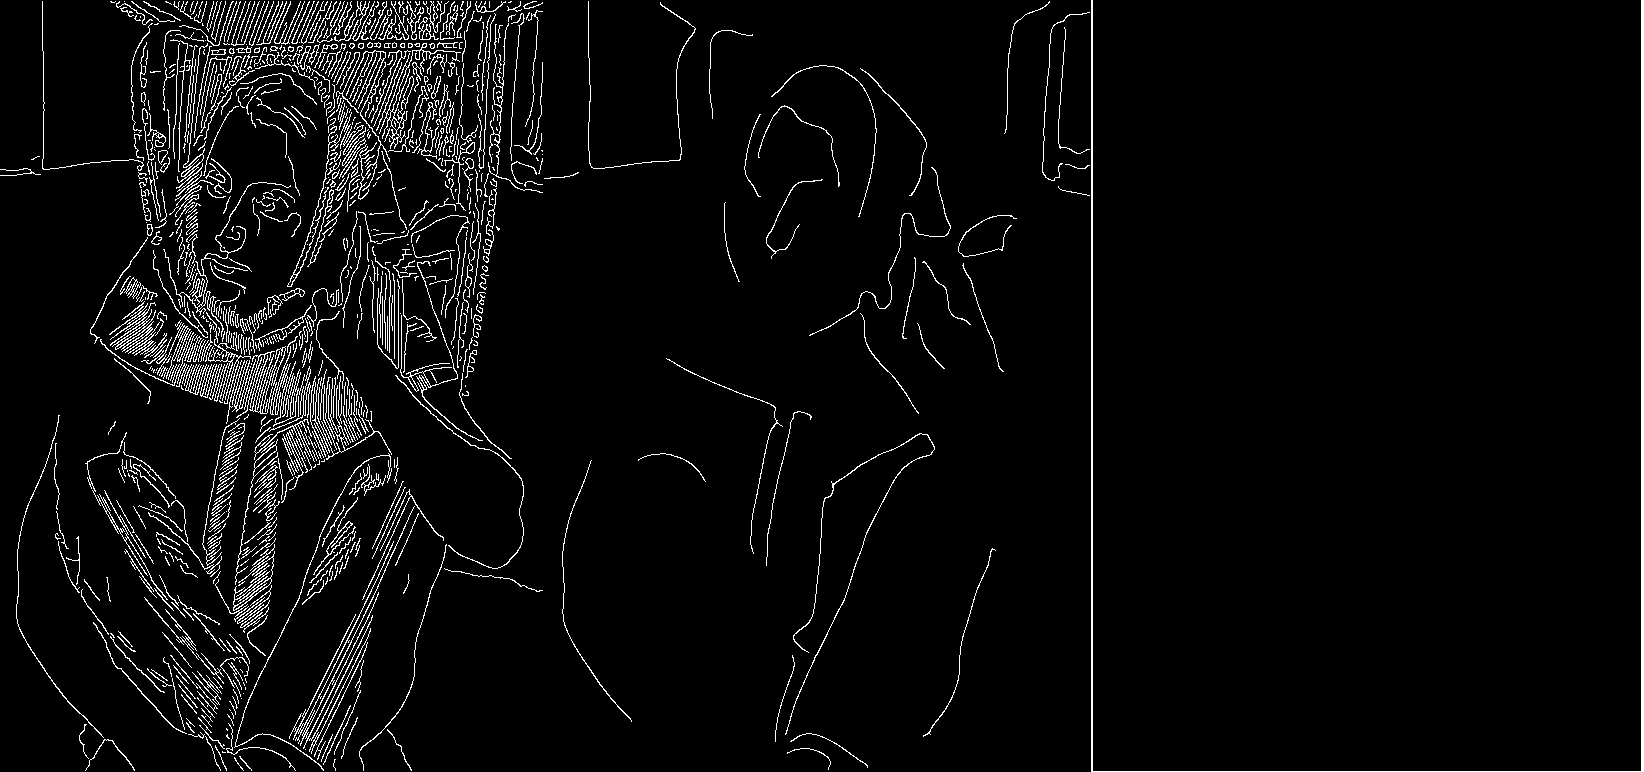
\includegraphics[width=1.0\textwidth]{images/canny-edge-barbara}
  \caption{Resultatet av Canny kantdetktor}
  \label{fig:canny}
\end{figure}


\begin{figure}[h]
  \centering
  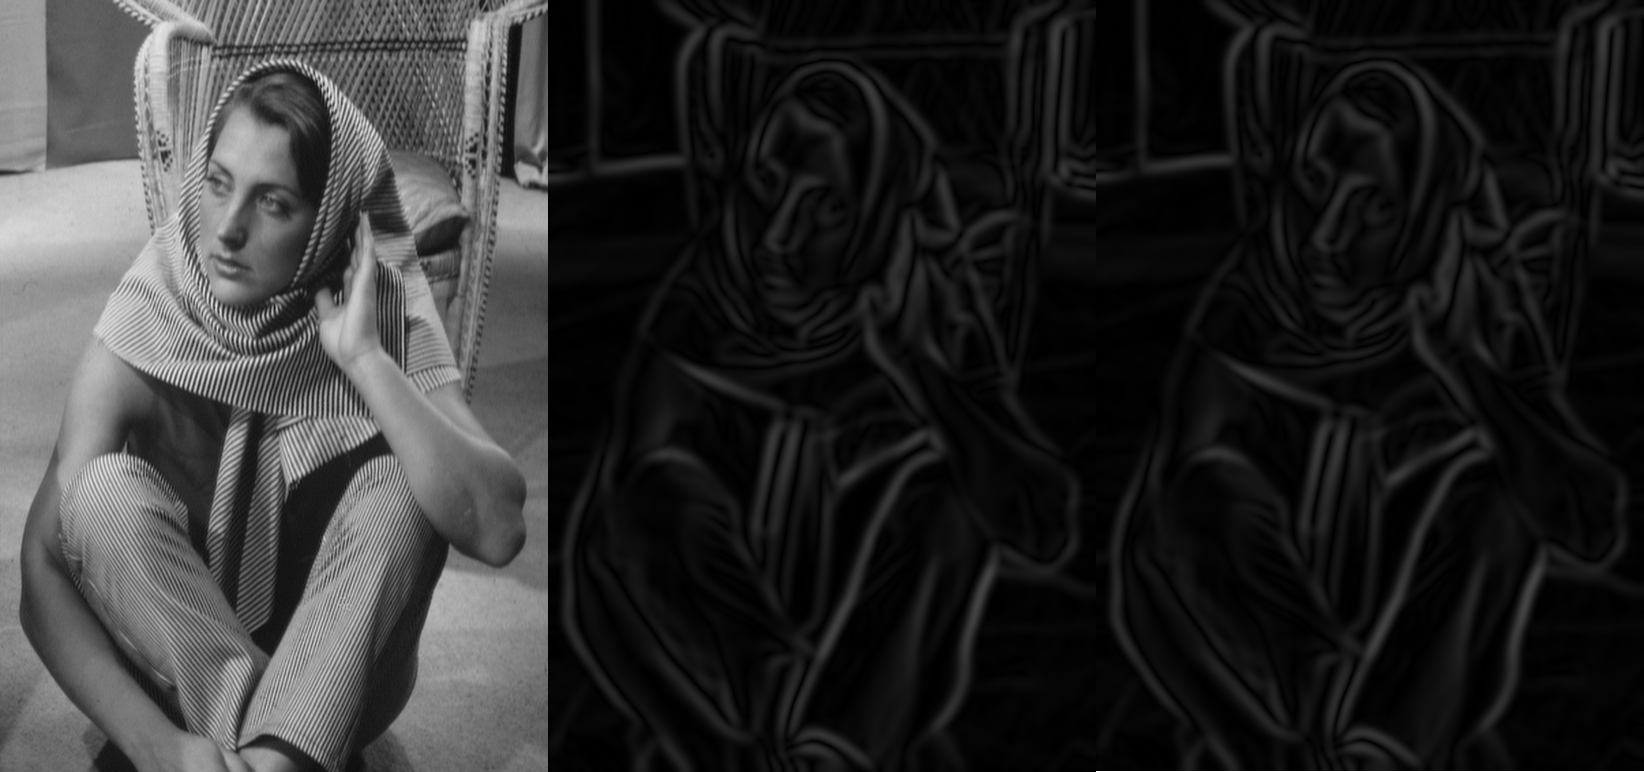
\includegraphics[width=1.0\textwidth]{images/barbara_prewitt_sobel}
  \caption{Resultat fra Sobel og Prewitt operator}
  \label{fig:sobprew}
\end{figure}

\begin{figure}[h]
  \centering
  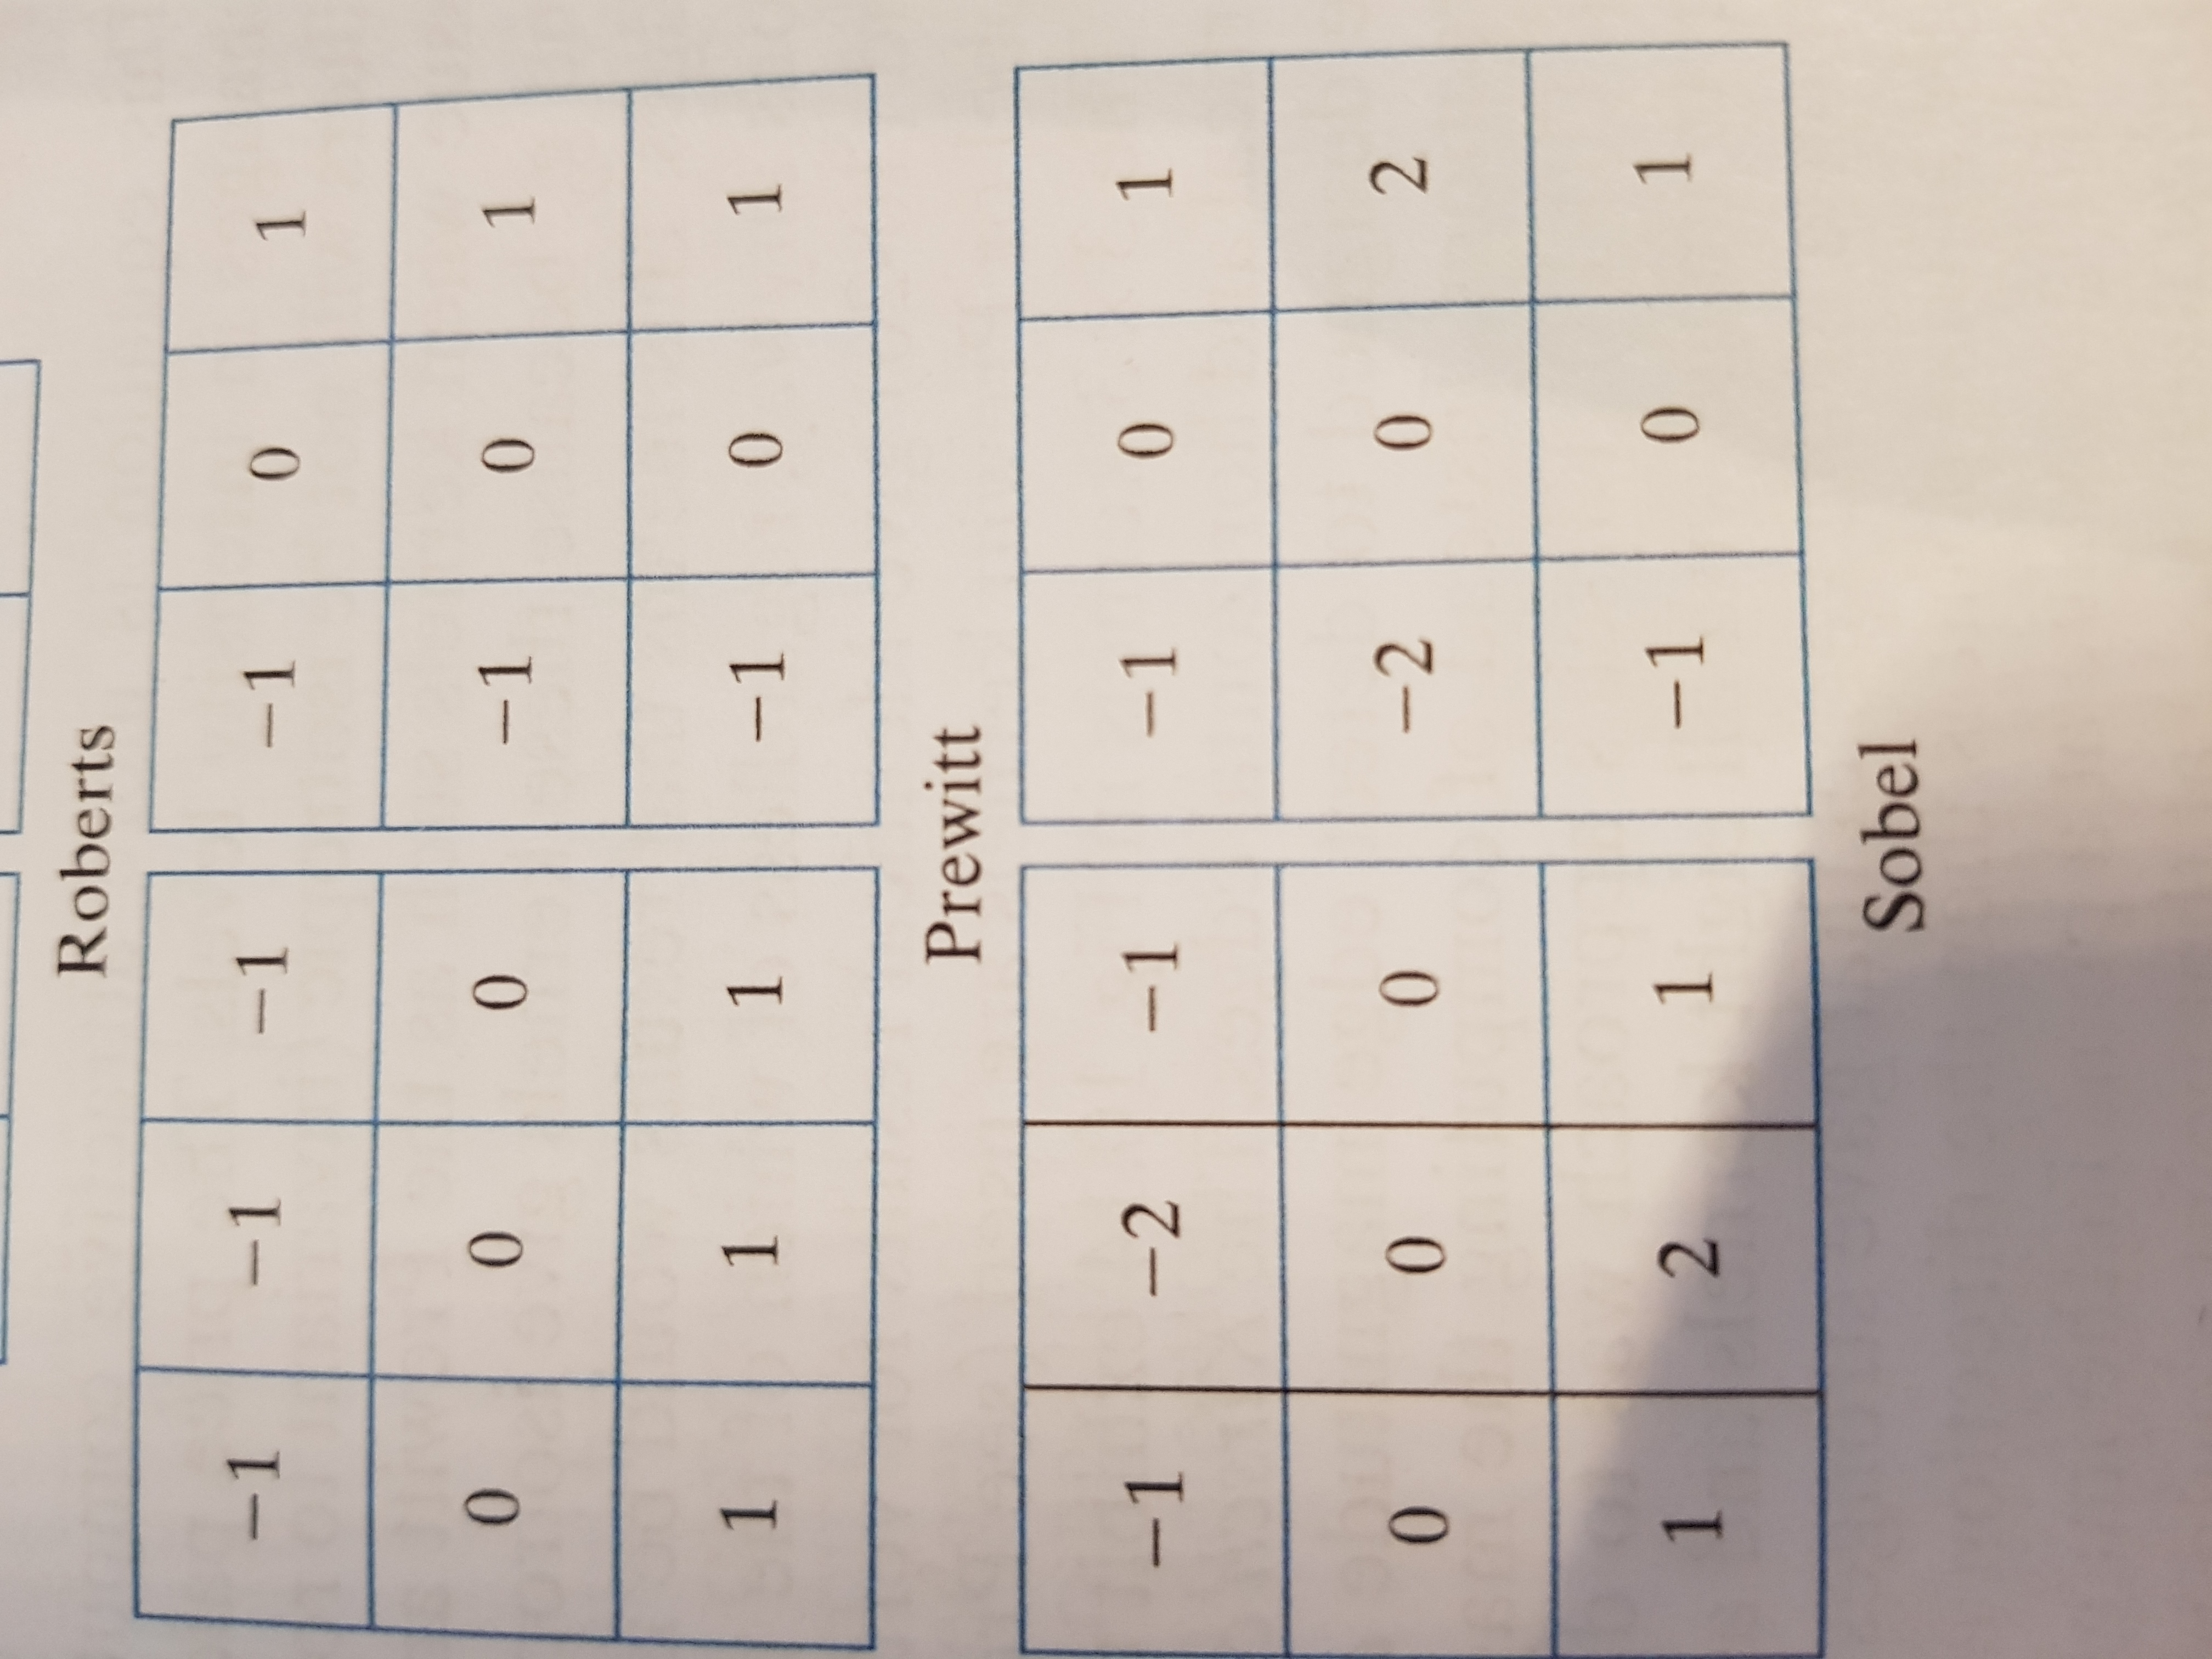
\includegraphics[width=0.5\textwidth, angle=270]{images/matrix}
  \caption{Sobel og Prewitt operatorer}
  \label{fig:mat}
\end{figure}

\end{document}